\section{Introduction}
The exploration of the ``weight space'' of neural network (NN) models, i.e., the high-dimensional space spanned by the model parameters of a population of trained NNs, allows us to gain insights into the inner workings of those models. 

%%%%%%%%%%%%%%%%%%%%%%%%%%%%%%%%%%%%%%%%%%%%%%%%%%%%%%%%%%%%%%%%%%%%%%%%%%%%
\begin{figure}[t!]
\centering
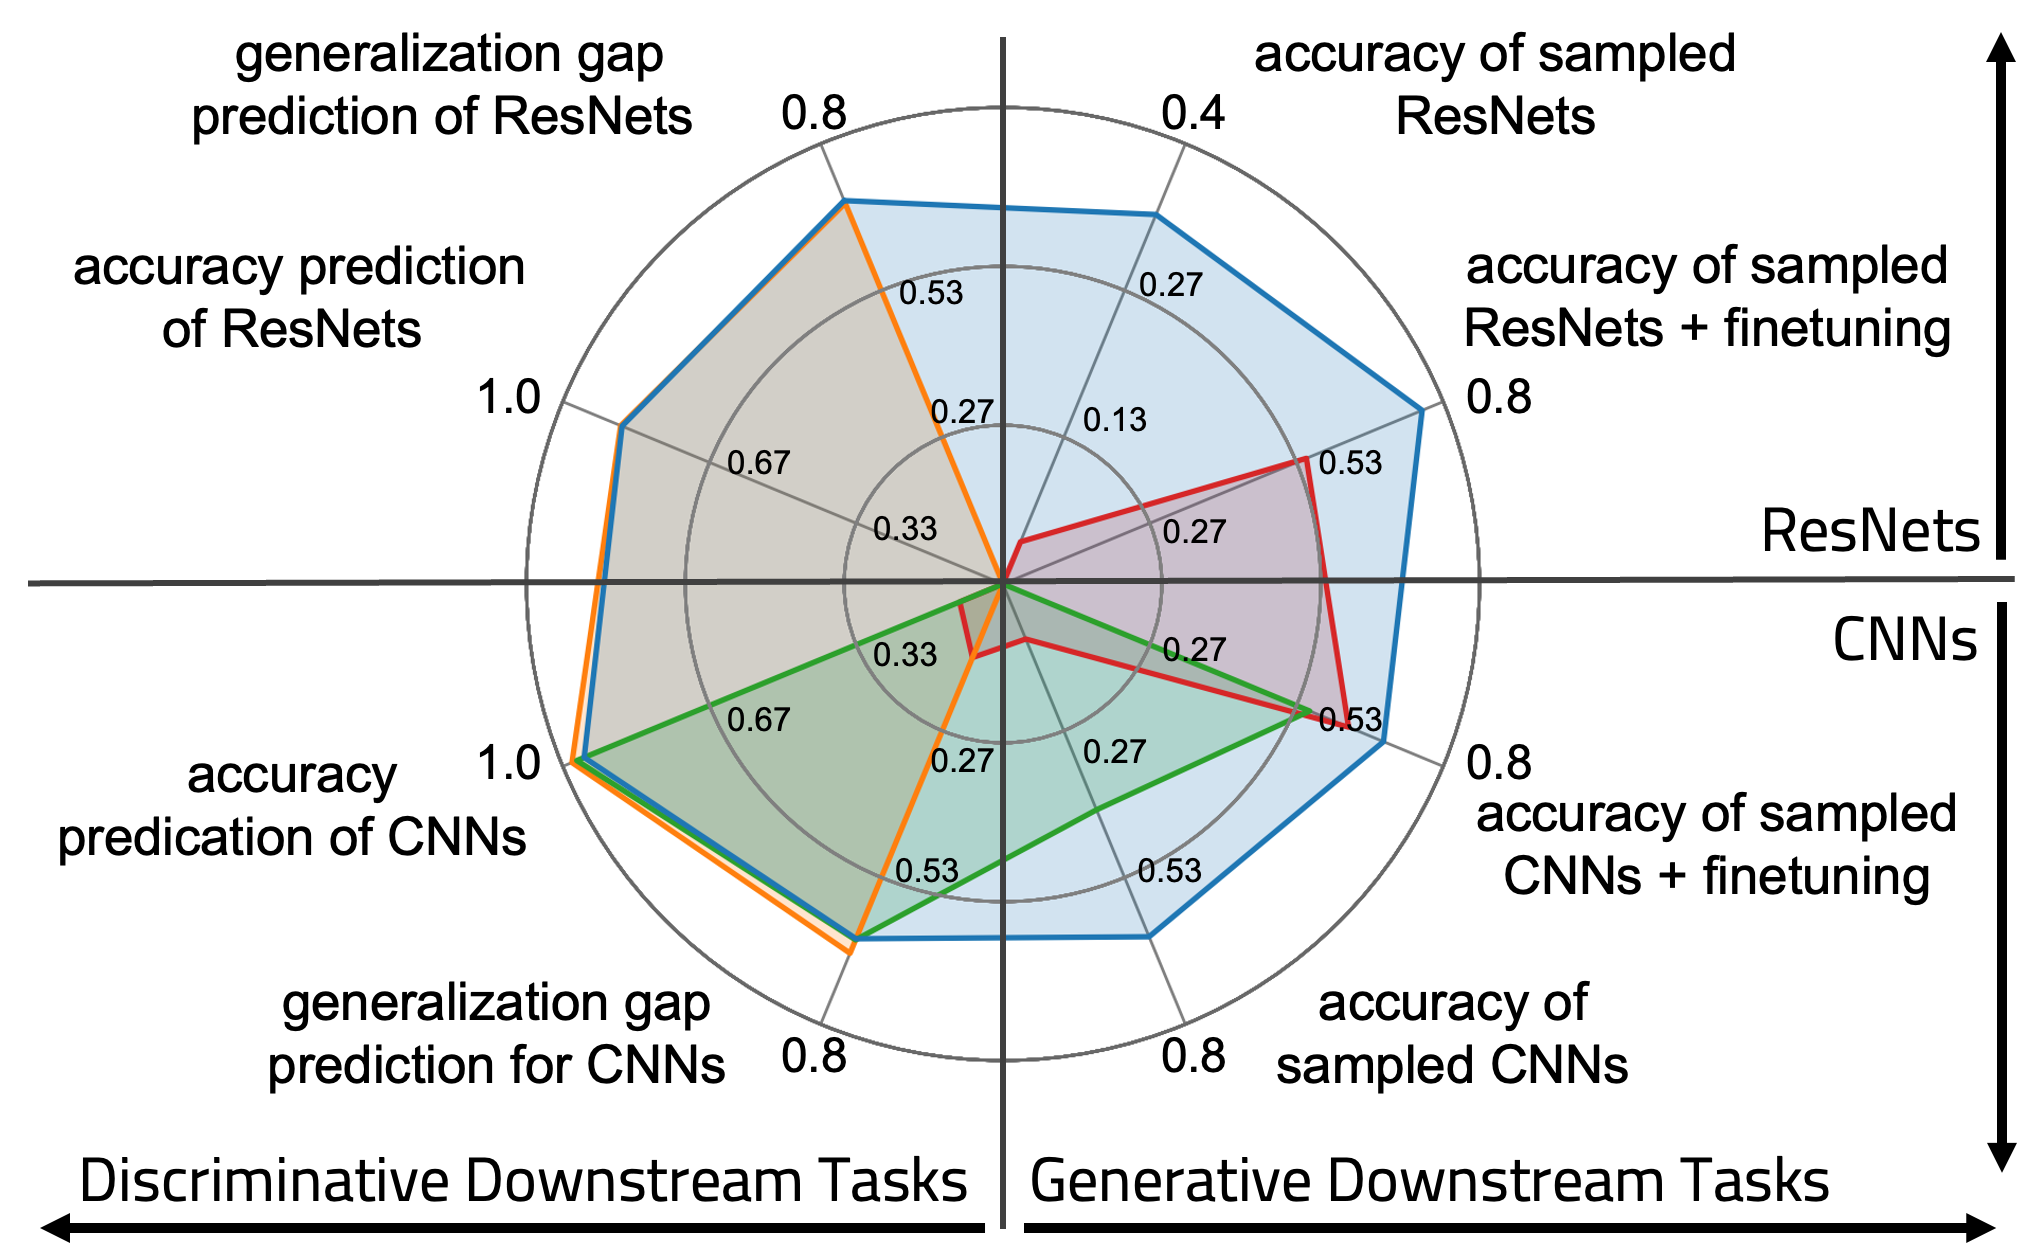
\includegraphics[width=1\columnwidth]{figures/radar_plot_overview_v12.png}
\vspace{-0.7cm}
\caption{Aggregated results of 56 experiments showing \textbf{(left:)} four discriminative downstream tasks in $R^2$, and (\textbf{right:}) four generative downstream tasks in accuracy, each evaluated on (\textbf{bottom:}) CNNs model zoos trained on 4 datasets (NMIST, SVHN, CIFAR-10, STL) and (\textbf{top:}) ResNet18 model zoos trained on three datasets (CIFAR-10, CIFAR-100, Tiny-ImageNet).  
%
The colors indicate performance of {\color{Red}\textbf{\texttt{Red:}}} raw NN weights, {\color{RedOrange}\textbf{\texttt{Orange:}}} weight statistics from \citet{unterthinerPredictingNeuralNetwork2020}, {\color{Green}\textbf{\texttt{Green:}}} trained \textit{hyper-representations} from \citet{schurholtSelfSupervisedRepresentationLearning2021, schurholtHyperRepresentationsGenerativeModels2022}, and {\color{Blue}\textbf{\texttt{Blue:}}} \ourmethod (ours).
%
While some methods perform well on specific tasks, or are restricted by the size of the underlying models, \ourmethod can deliver excellent performance on all tasks and model sizes.
}
\vspace{-0.6cm}
\label{fig:radar_plot_overview}
\end{figure}
%%%%%%%%%%%%%%%%%%%%%%%%%%%%%%%%%%%%%%%%%%%%%%%%%%%%%%%%%%%%%%%%%%%%%%%%%%%%

\vspace{0.1cm}

In the discriminative context, previous works aim to link weight space properties to properties such as model quality, generalization gap, or hyperparameters, using either the margin distribution \citep{yakTaskArchitectureIndependentGeneralization2019,jiangPredictingGeneralizationGap2019}, graph topology features \citep{corneanuComputingTestingError2020}, or eigenvalue decompositions of weight matrices \citep{martinTraditionalHeavyTailedSelf2019,MM20_SDM,martinImplicitSelfregularizationDeep2021,martinPredictingTrendsQuality2021}.
Some works learn classifiers to map between statistics of weights and model properties \citep{eilertsenClassifyingClassifierDissecting2020, unterthinerPredictingNeuralNetwork2020},
or learn lower-dimensional manifolds to infer NN model properties \citep{schurholtSelfSupervisedRepresentationLearning2021}.

%%%%%%%%%%%%%%%%%%%%%%%%%%%%%%%%%%%%%%%%%%%%%%%%%%%%%%%%%%%%%%%%%%%%%%%%%%%%
\begin{figure*}[t!]
\centering
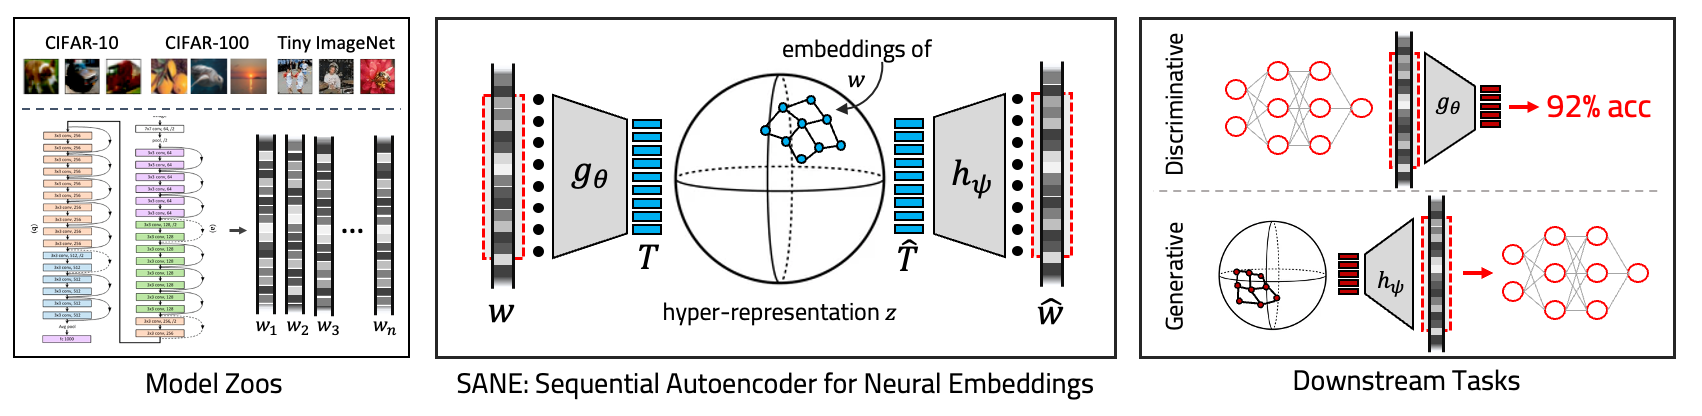
\includegraphics[width=0.75\paperwidth]{figures/approach_overview_2.png}
\vspace{-0.55cm}
\caption{
Given model zoos trained on different classification tasks, we extract and sequentialize the model weights. \ourmethod trains \textit{hyper-representations} on 
weights subsequences, i.e., individual layers.
\ourmethod can be used for multiple downstream tasks, either using the encoder for discriminative tasks such as the prediction of model accuracy, or the decoder for generative tasks such as sampling of new models.
}
\vspace{-0.3cm}
\label{fig:approach_overview}
\end{figure*}
%%%%%%%%%%%%%%%%%%%%%%%%%%%%%%%%%%%%%%%%%%%%%%%%%%%%%%%%%%%%%%%%%%%%%%%%%%%%

%
% generative
%
In the generative context, methods have been proposed to generate model weights using (Graph) HyperNetworks ~\citep{haHyperNetworks2016, zhangGraphHyperNetworksNeural2019, knyazevParameterPredictionUnseen2021}, Bayesian HyperNetworks \citep{deutschGeneratingNeuralNetworks2018}, HyperGANs \citep{ratzlaffHyperGANGenerativeModel2019}, and HyperTransformers \citep{zhmoginovHyperTransformerModelGeneration2022}.
These approaches have been used for tasks such as neural architecture search, model compression, ensembling, transfer learning, and meta-learning. They have in common that they derive their learning signal from the underlying (typically image) dataset. 
In contrast to these methods, 
so-called \textit{hyper-representations}~\citep{schurholtHyperRepresentationsGenerativeModels2022} learn a lower-dimensional representation directly from the weight space without the need to have access to data, e.g., the image dataset, to sample unseen NN models from that latent representation.



%
% our work
%
In this paper, we present \ourmethodlong (\ourmethod), an approach to learn task-agnostic representations of NN weight spaces capable of embedding individual NN models into a latent space to perform the above-mentioned discriminative or generative downstream tasks.
%
Our approach builds upon the idea of 
\textit{hyper-representations}~\citep{schurholtSelfSupervisedRepresentationLearning2021, schurholtHyperRepresentationsGenerativeModels2022}, which learn a lower-dimensional representation $z$ from a population of NN models. 
This is accomplished by auto-encoding their flattened weight vectors $w_i$ through a transformer architecture, with the bottleneck acting as a lower-dimensional embedding $z_i$ of each NN model. 
While the \textit{hyper-representation} method promises to be useful for discriminative and generative tasks, until now, separate \textit{hyper-representations} had to be trained specifically for either discriminative or generative tasks. 
Additionally, existing approaches have a major shortcoming: the underlying encoder-decoder model has to embed the entire flattened weight vectors $w_i$ at once into the learned lower-dimensional representation $z$. 
%
This drastically limits the size of NNs that can be embedded.
\ourmethod addresses these limitations by decomposing the entire weight vector $w_i$ into layers or smaller subsets, and then sequentially processes them. 
Instead of encoding the entire NN model by one embedding, \ourmethod encodes a potentially very large NN as multiple embeddings. 
%
The change from processing the entire flattened weight vector to subsets of weights is motivated by \citet{martinRethinkingGeneralizationRequires2019,martinImplicitSelfregularizationDeep2021}, who showed that global model information is preserved in the layer-wise components of NNs. 
An illustration of our approach can be found in Fig.~\ref{fig:approach_overview}.\looseness-1

%
To evaluate \ourmethod, we analyze how NN embeddings encoded by \ourmethod behave in comparison to \citet{martinRethinkingGeneralizationRequires2019,martinImplicitSelfregularizationDeep2021} quality measures. 
We show that some of these weight matrix quality metrics show similar characteristics as the embeddings produced by \ourmethod. 
This holds not only for held-out NN models of the model zoo used for training \ourmethod but also for NN models of out-of-distribution model zoos with different architectures and training data.
% 
Further, we demonstrate that \ourmethod can learn \textit{hyper-representations} of much larger NN models, and so it makes them applicable to real-world problems. 
%
In particular, the models in the ResNet model zoo used for training are three orders of magnitudes larger than all model zoos used for \textit{hyper-representation} learning in previous works. 
While previous \textit{hyper-representation} learning methods were structurally constrained to encode the entire NN model at once, \ourmethod is scalable by applying its sequential approach to encode layers or subsets of weights into hyper-representation embeddings.
While we demonstrate scaling up to ResNet-101 models, \ourmethod is not fundamentally limited to that size.
%
Finally, we evaluate \ourmethod on both discriminative and generative downstream tasks.
For discriminate tasks, we evaluate on six model zoos by linear-probing for properties of the underlying NN models. 
For generative tasks, we evaluate on seven model zoos by sampling targeted model weights for initialization and transfer learning. 

% downstream task results 
We provide an aggregated overview of our results in Fig.~\ref{fig:radar_plot_overview}. 
On very small CNN models (evaluated on MNIST, SVHN, CIFAR-10, and STL, which we include for comparison with prior work), \ourmethod performs as well as previous state-of-the-art (SOTA) in discriminative tasks. In generative downstream tasks, \ourmethod outperforms SOTA by 25\% in accuracy for initialization on the same task and 17\% in accuracy for finetuning to new tasks.
%
On larger models such as ResNets (evaluated on CIFAR-10, CIFAR-100, Tiny-ImageNet, which were beyond the capabilities of prior work), we show results comparable to baselines for discriminative downstream tasks, and we report outperformance to baselines for generative downstream tasks by 31\% for initialization and 28\% for finetuning to new tasks. 
%
Additionally, we show that \ourmethod can sample targeted models by prompting with different architectures than it used for training. These sampled models can outperform models trained from scratch on the prompted architecture. Code is available at \href{https://github.com/HSG-AIML/SANE}{github.com/HSG-AIML/SANE}.\looseness-1

